\documentclass[1p]{elsarticle_modified}
%\bibliographystyle{elsarticle-num}

%\usepackage[colorlinks]{hyperref}
%\usepackage{abbrmath_seonhwa} %\Abb, \Ascr, \Acal ,\Abf, \Afrak
\usepackage{amsfonts}
\usepackage{amssymb}
\usepackage{amsmath}
\usepackage{amsthm}
\usepackage{scalefnt}
\usepackage{amsbsy}
\usepackage{kotex}
\usepackage{caption}
\usepackage{subfig}
\usepackage{color}
\usepackage{graphicx}
\usepackage{xcolor} %% white, black, red, green, blue, cyan, magenta, yellow
\usepackage{float}
\usepackage{setspace}
\usepackage{hyperref}

\usepackage{tikz}
\usetikzlibrary{arrows}

\usepackage{multirow}
\usepackage{array} % fixed length table
\usepackage{hhline}

%%%%%%%%%%%%%%%%%%%%%
\makeatletter
\renewcommand*\env@matrix[1][\arraystretch]{%
	\edef\arraystretch{#1}%
	\hskip -\arraycolsep
	\let\@ifnextchar\new@ifnextchar
	\array{*\c@MaxMatrixCols c}}
\makeatother %https://tex.stackexchange.com/questions/14071/how-can-i-increase-the-line-spacing-in-a-matrix
%%%%%%%%%%%%%%%

\usepackage[normalem]{ulem}

\newcommand{\msout}[1]{\ifmmode\text{\sout{\ensuremath{#1}}}\else\sout{#1}\fi}
%SOURCE: \msout is \stkout macro in https://tex.stackexchange.com/questions/20609/strikeout-in-math-mode

\newcommand{\cancel}[1]{
	\ifmmode
	{\color{red}\msout{#1}}
	\else
	{\color{red}\sout{#1}}
	\fi
}

\newcommand{\add}[1]{
	{\color{blue}\uwave{#1}}
}

\newcommand{\replace}[2]{
	\ifmmode
	{\color{red}\msout{#1}}{\color{blue}\uwave{#2}}
	\else
	{\color{red}\sout{#1}}{\color{blue}\uwave{#2}}
	\fi
}

\newcommand{\Sol}{\mathcal{S}} %segment
\newcommand{\D}{D} %diagram
\newcommand{\A}{\mathcal{A}} %arc


%%%%%%%%%%%%%%%%%%%%%%%%%%%%%5 test

\def\sl{\operatorname{\textup{SL}}(2,\Cbb)}
\def\psl{\operatorname{\textup{PSL}}(2,\Cbb)}
\def\quan{\mkern 1mu \triangleright \mkern 1mu}

\theoremstyle{definition}
\newtheorem{thm}{Theorem}[section]
\newtheorem{prop}[thm]{Proposition}
\newtheorem{lem}[thm]{Lemma}
\newtheorem{ques}[thm]{Question}
\newtheorem{cor}[thm]{Corollary}
\newtheorem{defn}[thm]{Definition}
\newtheorem{exam}[thm]{Example}
\newtheorem{rmk}[thm]{Remark}
\newtheorem{alg}[thm]{Algorithm}

\newcommand{\I}{\sqrt{-1}}
\begin{document}

%\begin{frontmatter}
%
%\title{Boundary parabolic representations of knots up to 8 crossings}
%
%%% Group authors per affiliation:
%\author{Yunhi Cho} 
%\address{Department of Mathematics, University of Seoul, Seoul, Korea}
%\ead{yhcho@uos.ac.kr}
%
%
%\author{Seonhwa Kim} %\fnref{s_kim}}
%\address{Center for Geometry and Physics, Institute for Basic Science, Pohang, 37673, Korea}
%\ead{ryeona17@ibs.re.kr}
%
%\author{Hyuk Kim}
%\address{Department of Mathematical Sciences, Seoul National University, Seoul 08826, Korea}
%\ead{hyukkim@snu.ac.kr}
%
%\author{Seokbeom Yoon}
%\address{Department of Mathematical Sciences, Seoul National University, Seoul, 08826,  Korea}
%\ead{sbyoon15@snu.ac.kr}
%
%\begin{abstract}
%We find all boundary parabolic representation of knots up to 8 crossings.
%
%\end{abstract}
%\begin{keyword}
%    \MSC[2010] 57M25 
%\end{keyword}
%
%\end{frontmatter}

%\linenumbers
%\tableofcontents
%
\newcommand\colored[1]{\textcolor{white}{\rule[-0.35ex]{0.8em}{1.4ex}}\kern-0.8em\color{red} #1}%
%\newcommand\colored[1]{\textcolor{white}{ #1}\kern-2.17ex	\textcolor{white}{ #1}\kern-1.81ex	\textcolor{white}{ #1}\kern-2.15ex\color{red}#1	}

{\Large $\underline{12n_{0617}~(K12n_{0617})}$}

\setlength{\tabcolsep}{10pt}
\renewcommand{\arraystretch}{1.6}
\vspace{1cm}\begin{tabular}{m{100pt}>{\centering\arraybackslash}m{274pt}}
\multirow{5}{120pt}{
	\centering
	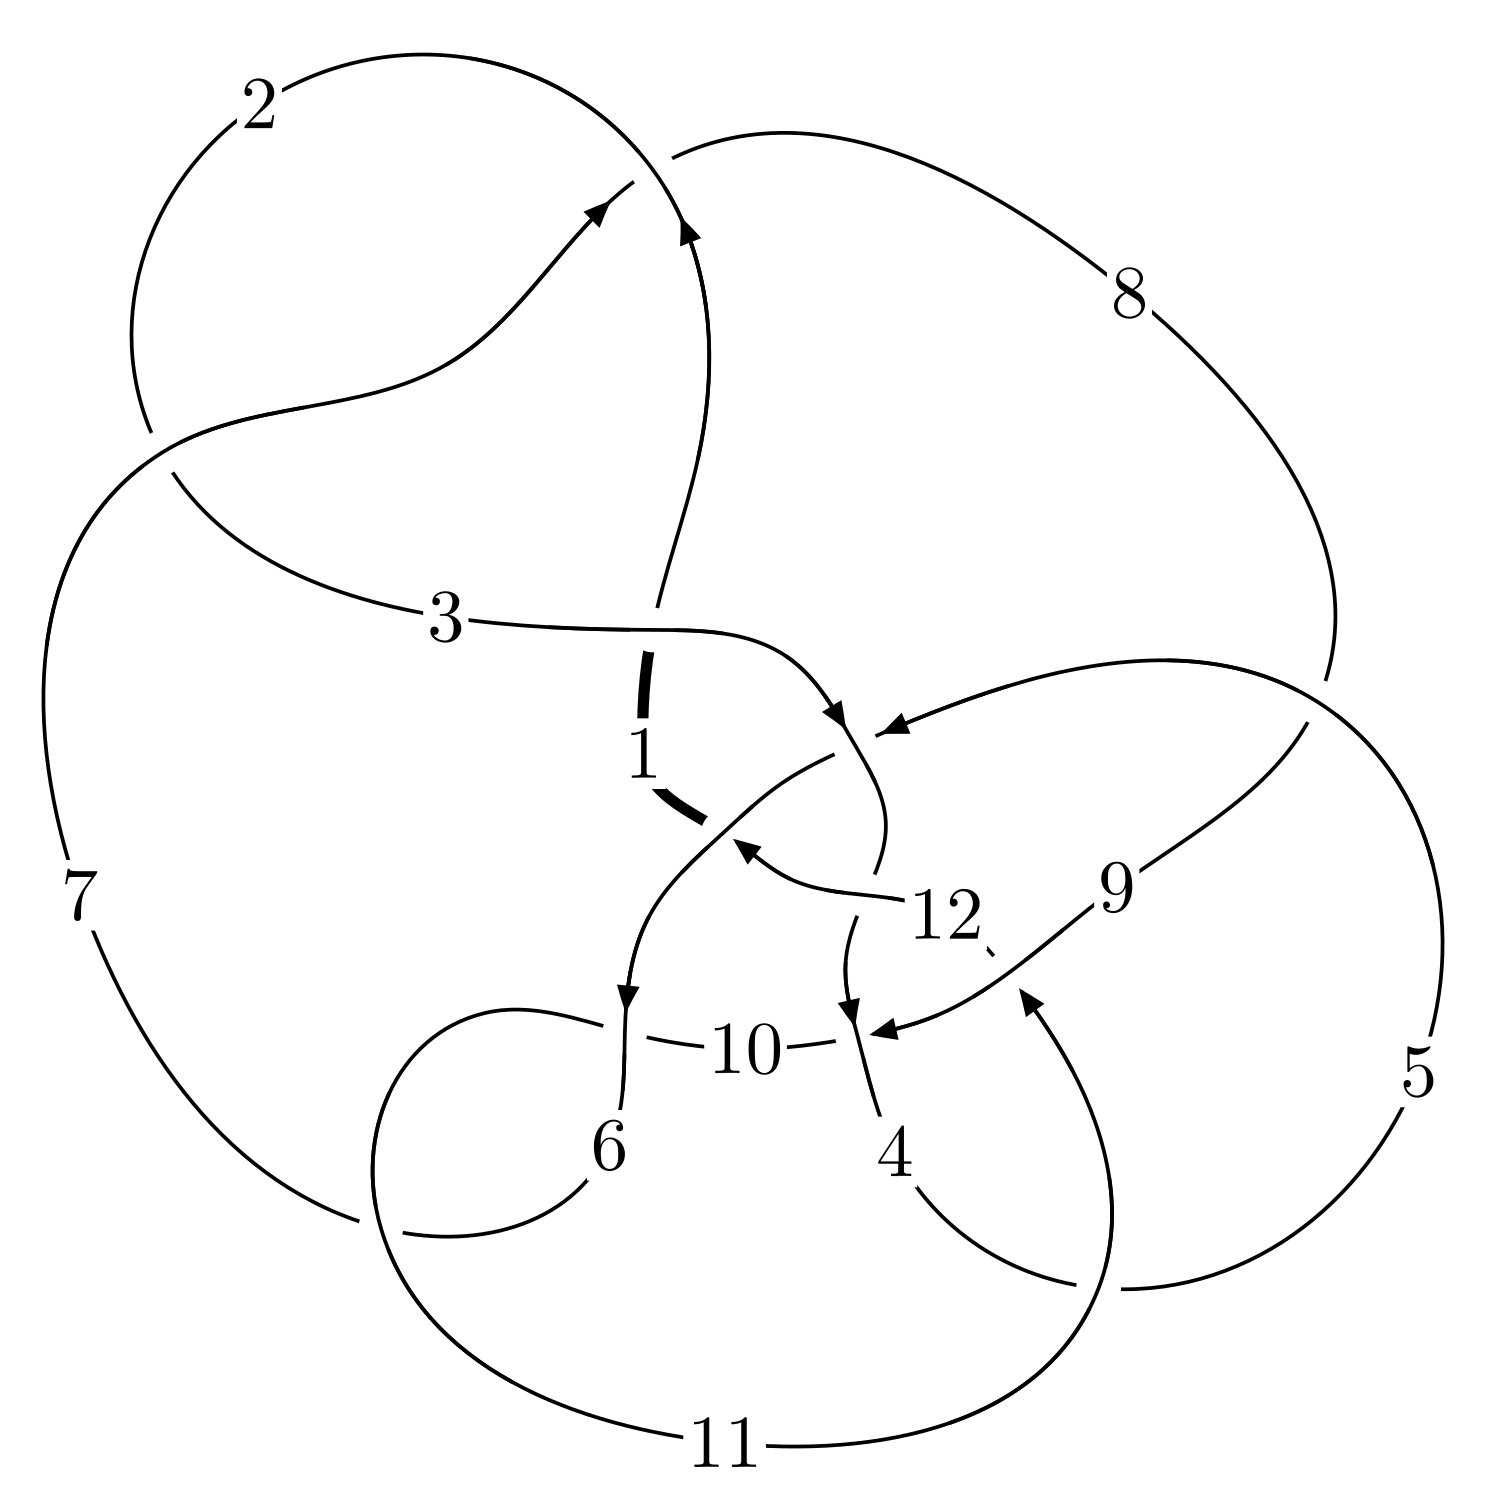
\includegraphics[width=112pt]{../../../GIT/diagram.site/Diagrams/png/2706_12n_0617.png}\\
\ \ \ A knot diagram\footnotemark}&
\allowdisplaybreaks
\textbf{Linearized knot diagam} \\
\cline{2-2}
 &
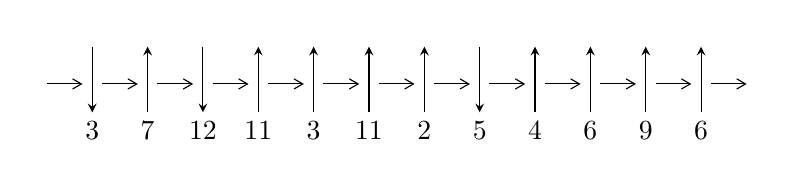
\begin{tikzpicture}[x=20pt, y=17pt]
	% nodes
	\node (C0) at (0, 0) {};
	\node (C1) at (1, 0) {};
	\node (C1U) at (1, +1) {};
	\node (C1D) at (1, -1) {3};

	\node (C2) at (2, 0) {};
	\node (C2U) at (2, +1) {};
	\node (C2D) at (2, -1) {7};

	\node (C3) at (3, 0) {};
	\node (C3U) at (3, +1) {};
	\node (C3D) at (3, -1) {12};

	\node (C4) at (4, 0) {};
	\node (C4U) at (4, +1) {};
	\node (C4D) at (4, -1) {11};

	\node (C5) at (5, 0) {};
	\node (C5U) at (5, +1) {};
	\node (C5D) at (5, -1) {3};

	\node (C6) at (6, 0) {};
	\node (C6U) at (6, +1) {};
	\node (C6D) at (6, -1) {11};

	\node (C7) at (7, 0) {};
	\node (C7U) at (7, +1) {};
	\node (C7D) at (7, -1) {2};

	\node (C8) at (8, 0) {};
	\node (C8U) at (8, +1) {};
	\node (C8D) at (8, -1) {5};

	\node (C9) at (9, 0) {};
	\node (C9U) at (9, +1) {};
	\node (C9D) at (9, -1) {4};

	\node (C10) at (10, 0) {};
	\node (C10U) at (10, +1) {};
	\node (C10D) at (10, -1) {6};

	\node (C11) at (11, 0) {};
	\node (C11U) at (11, +1) {};
	\node (C11D) at (11, -1) {9};

	\node (C12) at (12, 0) {};
	\node (C12U) at (12, +1) {};
	\node (C12D) at (12, -1) {6};
	\node (C13) at (13, 0) {};

	% arrows
	\draw[->,>={angle 60}]
	(C0) edge (C1) (C1) edge (C2) (C2) edge (C3) (C3) edge (C4) (C4) edge (C5) (C5) edge (C6) (C6) edge (C7) (C7) edge (C8) (C8) edge (C9) (C9) edge (C10) (C10) edge (C11) (C11) edge (C12) (C12) edge (C13) ;	\draw[->,>=stealth]
	(C1U) edge (C1D) (C2D) edge (C2U) (C3U) edge (C3D) (C4D) edge (C4U) (C5D) edge (C5U) (C6D) edge (C6U) (C7D) edge (C7U) (C8U) edge (C8D) (C9D) edge (C9U) (C10D) edge (C10U) (C11D) edge (C11U) (C12D) edge (C12U) ;
	\end{tikzpicture} \\
\hhline{~~} \\& 
\textbf{Solving Sequence} \\ \cline{2-2} 
 &
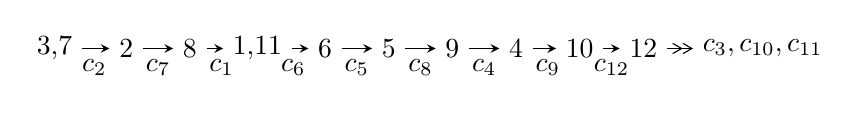
\begin{tikzpicture}[x=23pt, y=7pt]
	% node
	\node (A0) at (-1/8, 0) {3,7};
	\node (A1) at (1, 0) {2};
	\node (A2) at (2, 0) {8};
	\node (A3) at (49/16, 0) {1,11};
	\node (A4) at (33/8, 0) {6};
	\node (A5) at (41/8, 0) {5};
	\node (A6) at (49/8, 0) {9};
	\node (A7) at (57/8, 0) {4};
	\node (A8) at (65/8, 0) {10};
	\node (A9) at (73/8, 0) {12};
	\node (C1) at (1/2, -1) {$c_{2}$};
	\node (C2) at (3/2, -1) {$c_{7}$};
	\node (C3) at (5/2, -1) {$c_{1}$};
	\node (C4) at (29/8, -1) {$c_{6}$};
	\node (C5) at (37/8, -1) {$c_{5}$};
	\node (C6) at (45/8, -1) {$c_{8}$};
	\node (C7) at (53/8, -1) {$c_{4}$};
	\node (C8) at (61/8, -1) {$c_{9}$};
	\node (C9) at (69/8, -1) {$c_{12}$};
	\node (A10) at (11, 0) {$c_{3},c_{10},c_{11}$};

	% edge
	\draw[->,>=stealth]	
	(A0) edge (A1) (A1) edge (A2) (A2) edge (A3) (A3) edge (A4) (A4) edge (A5) (A5) edge (A6) (A6) edge (A7) (A7) edge (A8) (A8) edge (A9) ;
	\draw[->>,>={angle 60}]	
	(A9) edge (A10);
\end{tikzpicture} \\ 

\end{tabular} \\

\footnotetext{
The image of knot diagram is generated by the software ``\textbf{Draw programme}" developed by Andrew Bartholomew(\url{http://www.layer8.co.uk/maths/draw/index.htm\#Running-draw}), where we modified some parts for our purpose(\url{https://github.com/CATsTAILs/LinksPainter}).
}\phantom \\ \newline 
\centering \textbf{Ideals for irreducible components\footnotemark of $X_{\text{par}}$} 
 
\begin{align*}
I^u_{1}&=\langle 
-4.03528\times10^{29} u^{18}+2.20603\times10^{29} u^{17}+\cdots+1.42881\times10^{32} b-1.94886\times10^{32},\\
\phantom{I^u_{1}}&\phantom{= \langle  }-1.72871\times10^{32} u^{18}+8.76867\times10^{31} u^{17}+\cdots+4.27215\times10^{34} a-1.13938\times10^{35},\\
\phantom{I^u_{1}}&\phantom{= \langle  }u^{19}+7 u^{17}+\cdots+1241 u+299\rangle \\
I^u_{2}&=\langle 
341324 u^{18}+743649 u^{17}+\cdots+1775197 b-6939035,\\
\phantom{I^u_{2}}&\phantom{= \langle  }-4528372 u^{18}-453288 u^{17}+\cdots+5325591 a-8838485,\;u^{19}+9 u^{17}+\cdots+5 u-3\rangle \\
I^u_{3}&=\langle 
b+1,\;a+u+1,\;u^2+u+1\rangle \\
\\
\end{align*}
\raggedright * 3 irreducible components of $\dim_{\mathbb{C}}=0$, with total 40 representations.\\
\footnotetext{All coefficients of polynomials are rational numbers. But the coefficients are sometimes approximated in decimal forms when there is not enough margin.}
\newpage
\renewcommand{\arraystretch}{1}
\centering \section*{I. $I^u_{1}= \langle -4.04\times10^{29} u^{18}+2.21\times10^{29} u^{17}+\cdots+1.43\times10^{32} b-1.95\times10^{32},\;-1.73\times10^{32} u^{18}+8.77\times10^{31} u^{17}+\cdots+4.27\times10^{34} a-1.14\times10^{35},\;u^{19}+7 u^{17}+\cdots+1241 u+299 \rangle$}
\flushleft \textbf{(i) Arc colorings}\\
\begin{tabular}{m{7pt} m{180pt} m{7pt} m{180pt} }
\flushright $a_{3}=$&$\begin{pmatrix}1\\0\end{pmatrix}$ \\
\flushright $a_{7}=$&$\begin{pmatrix}0\\u\end{pmatrix}$ \\
\flushright $a_{2}=$&$\begin{pmatrix}1\\u^2\end{pmatrix}$ \\
\flushright $a_{8}=$&$\begin{pmatrix}u\\u^3+u\end{pmatrix}$ \\
\flushright $a_{1}=$&$\begin{pmatrix}u^2+1\\u^2\end{pmatrix}$ \\
\flushright $a_{11}=$&$\begin{pmatrix}0.00404647 u^{18}-0.00205252 u^{17}+\cdots+5.01173 u+2.66701\\0.00282422 u^{18}-0.00154396 u^{17}+\cdots+3.08557 u+1.36397\end{pmatrix}$ \\
\flushright $a_{6}=$&$\begin{pmatrix}0.00155291 u^{18}-0.00147152 u^{17}+\cdots+1.33246 u+0.620489\\0.0000864825 u^{18}-0.0000717914 u^{17}+\cdots+0.294414 u-0.189493\end{pmatrix}$ \\
\flushright $a_{5}=$&$\begin{pmatrix}0.00146643 u^{18}-0.00139973 u^{17}+\cdots+1.03805 u+0.809982\\0.0000864825 u^{18}-0.0000717914 u^{17}+\cdots+0.294414 u-0.189493\end{pmatrix}$ \\
\flushright $a_{9}=$&$\begin{pmatrix}0.000967454 u^{18}-0.000263588 u^{17}+\cdots+2.28928 u+0.510179\\-0.00189360 u^{18}+0.00123884 u^{17}+\cdots-1.20770 u-0.672255\end{pmatrix}$ \\
\flushright $a_{4}=$&$\begin{pmatrix}-0.00114874 u^{18}+0.000504223 u^{17}+\cdots-2.10077 u+0.100181\\-0.00200460 u^{18}+0.00203579 u^{17}+\cdots-2.29498 u-0.839146\end{pmatrix}$ \\
\flushright $a_{10}=$&$\begin{pmatrix}-0.00755089 u^{18}+0.00505904 u^{17}+\cdots-8.55381 u-3.61658\\-0.00579600 u^{18}+0.00405386 u^{17}+\cdots-6.14874 u-2.35891\end{pmatrix}$ \\
\flushright $a_{12}=$&$\begin{pmatrix}0.00349992 u^{18}-0.00250692 u^{17}+\cdots+4.15098 u+2.32935\\0.00305515 u^{18}-0.00208189 u^{17}+\cdots+3.55304 u+1.16410\end{pmatrix}$\\&\end{tabular}
\flushleft \textbf{(ii) Obstruction class $= -1$}\\~\\
\flushleft \textbf{(iii) Cusp Shapes $= 0.0112722 u^{18}-0.00351862 u^{17}+\cdots+14.6963 u+17.4566$}\\~\\
\newpage\renewcommand{\arraystretch}{1}
\flushleft \textbf{(iv) u-Polynomials at the component}\newline \\
\begin{tabular}{m{50pt}|m{274pt}}
Crossings & \hspace{64pt}u-Polynomials at each crossing \\
\hline $$\begin{aligned}c_{1}\end{aligned}$$&$\begin{aligned}
&u^{19}+14 u^{18}+\cdots+674775 u-89401
\end{aligned}$\\
\hline $$\begin{aligned}c_{2},c_{7}\end{aligned}$$&$\begin{aligned}
&u^{19}+7 u^{17}+\cdots+1241 u-299
\end{aligned}$\\
\hline $$\begin{aligned}c_{3}\end{aligned}$$&$\begin{aligned}
&u^{19}-5 u^{18}+\cdots+393 u-39
\end{aligned}$\\
\hline $$\begin{aligned}c_{4}\end{aligned}$$&$\begin{aligned}
&u^{19}-39 u^{17}+\cdots-7472 u+3053
\end{aligned}$\\
\hline $$\begin{aligned}c_{5}\end{aligned}$$&$\begin{aligned}
&u^{19}- u^{18}+\cdots+1014 u-111
\end{aligned}$\\
\hline $$\begin{aligned}c_{6},c_{10}\end{aligned}$$&$\begin{aligned}
&u^{19}+3 u^{18}+\cdots-360 u+108
\end{aligned}$\\
\hline $$\begin{aligned}c_{8}\end{aligned}$$&$\begin{aligned}
&u^{19}-4 u^{18}+\cdots+783 u-789
\end{aligned}$\\
\hline $$\begin{aligned}c_{9}\end{aligned}$$&$\begin{aligned}
&u^{19}+u^{18}+\cdots+3474 u+4197
\end{aligned}$\\
\hline $$\begin{aligned}c_{11}\end{aligned}$$&$\begin{aligned}
&u^{19}+4 u^{18}+\cdots-12 u-3
\end{aligned}$\\
\hline $$\begin{aligned}c_{12}\end{aligned}$$&$\begin{aligned}
&u^{19}+23 u^{17}+\cdots-12 u-3
\end{aligned}$\\
\hline
\end{tabular}\\~\\
\newpage\renewcommand{\arraystretch}{1}
\flushleft \textbf{(v) Riley Polynomials at the component}\newline \\
\begin{tabular}{m{50pt}|m{274pt}}
Crossings & \hspace{64pt}Riley Polynomials at each crossing \\
\hline $$\begin{aligned}c_{1}\end{aligned}$$&$\begin{aligned}
&y^{19}-66 y^{18}+\cdots+286804528071 y-7992538801
\end{aligned}$\\
\hline $$\begin{aligned}c_{2},c_{7}\end{aligned}$$&$\begin{aligned}
&y^{19}+14 y^{18}+\cdots+674775 y-89401
\end{aligned}$\\
\hline $$\begin{aligned}c_{3}\end{aligned}$$&$\begin{aligned}
&y^{19}+7 y^{18}+\cdots+57963 y-1521
\end{aligned}$\\
\hline $$\begin{aligned}c_{4}\end{aligned}$$&$\begin{aligned}
&y^{19}-78 y^{18}+\cdots+41701500 y-9320809
\end{aligned}$\\
\hline $$\begin{aligned}c_{5}\end{aligned}$$&$\begin{aligned}
&y^{19}-47 y^{18}+\cdots+419250 y-12321
\end{aligned}$\\
\hline $$\begin{aligned}c_{6},c_{10}\end{aligned}$$&$\begin{aligned}
&y^{19}-37 y^{18}+\cdots-80568 y-11664
\end{aligned}$\\
\hline $$\begin{aligned}c_{8}\end{aligned}$$&$\begin{aligned}
&y^{19}-66 y^{18}+\cdots+164937 y-622521
\end{aligned}$\\
\hline $$\begin{aligned}c_{9}\end{aligned}$$&$\begin{aligned}
&y^{19}-47 y^{18}+\cdots+31022328 y-17614809
\end{aligned}$\\
\hline $$\begin{aligned}c_{11}\end{aligned}$$&$\begin{aligned}
&y^{19}-2 y^{18}+\cdots+156 y-9
\end{aligned}$\\
\hline $$\begin{aligned}c_{12}\end{aligned}$$&$\begin{aligned}
&y^{19}+46 y^{18}+\cdots+102 y-9
\end{aligned}$\\
\hline
\end{tabular}\\~\\
\newpage\flushleft \textbf{(vi) Complex Volumes and Cusp Shapes}
$$\begin{array}{c|c|c}  
\text{Solutions to }I^u_{1}& \I (\text{vol} + \sqrt{-1}CS) & \text{Cusp shape}\\
 \hline 
\begin{aligned}
u &= \phantom{-}0.791837 + 0.677469 I \\
a &= -0.619990 + 0.658481 I \\
b &= -1.173080 - 0.756067 I\end{aligned}
 & \phantom{-}3.59219 - 0.75835 I & \phantom{-}12.53082 - 1.44797 I \\ \hline\begin{aligned}
u &= \phantom{-}0.791837 - 0.677469 I \\
a &= -0.619990 - 0.658481 I \\
b &= -1.173080 + 0.756067 I\end{aligned}
 & \phantom{-}3.59219 + 0.75835 I & \phantom{-}12.53082 + 1.44797 I \\ \hline\begin{aligned}
u &= \phantom{-}0.668469 + 1.020450 I \\
a &= \phantom{-}0.517672 - 0.080176 I \\
b &= \phantom{-}1.98730 + 0.83213 I\end{aligned}
 & \phantom{-}3.00456 + 6.40703 I & \phantom{-}1.37835 - 6.31753 I \\ \hline\begin{aligned}
u &= \phantom{-}0.668469 - 1.020450 I \\
a &= \phantom{-}0.517672 + 0.080176 I \\
b &= \phantom{-}1.98730 - 0.83213 I\end{aligned}
 & \phantom{-}3.00456 - 6.40703 I & \phantom{-}1.37835 + 6.31753 I \\ \hline\begin{aligned}
u &= -0.709865 + 0.235609 I \\
a &= -1.24244 + 1.33477 I \\
b &= -1.233030 + 0.441203 I\end{aligned}
 & -1.78162 + 2.24100 I & \phantom{-}7.64182 - 5.49504 I \\ \hline\begin{aligned}
u &= -0.709865 - 0.235609 I \\
a &= -1.24244 - 1.33477 I \\
b &= -1.233030 - 0.441203 I\end{aligned}
 & -1.78162 - 2.24100 I & \phantom{-}7.64182 + 5.49504 I \\ \hline\begin{aligned}
u &= -0.443396 + 0.513943 I \\
a &= \phantom{-}0.464073 - 0.228663 I \\
b &= \phantom{-}0.114778 - 0.413169 I\end{aligned}
 & \phantom{-}0.81666 - 1.62841 I & \phantom{-}5.50356 + 4.37919 I \\ \hline\begin{aligned}
u &= -0.443396 - 0.513943 I \\
a &= \phantom{-}0.464073 + 0.228663 I \\
b &= \phantom{-}0.114778 + 0.413169 I\end{aligned}
 & \phantom{-}0.81666 + 1.62841 I & \phantom{-}5.50356 - 4.37919 I \\ \hline\begin{aligned}
u &= \phantom{-}0.220968 + 1.307740 I \\
a &= \phantom{-}0.559258 + 0.670454 I \\
b &= -0.221871 + 0.268759 I\end{aligned}
 & -5.42189 - 4.80173 I & \phantom{-}4.68015 + 6.13601 I \\ \hline\begin{aligned}
u &= \phantom{-}0.220968 - 1.307740 I \\
a &= \phantom{-}0.559258 - 0.670454 I \\
b &= -0.221871 - 0.268759 I\end{aligned}
 & -5.42189 + 4.80173 I & \phantom{-}4.68015 - 6.13601 I\\
 \hline 
 \end{array}$$\newpage$$\begin{array}{c|c|c}  
\text{Solutions to }I^u_{1}& \I (\text{vol} + \sqrt{-1}CS) & \text{Cusp shape}\\
 \hline 
\begin{aligned}
u &= \phantom{-}1.34390\phantom{ +0.000000I} \\
a &= -1.75903\phantom{ +0.000000I} \\
b &= -1.60303\phantom{ +0.000000I}\end{aligned}
 & \phantom{-}7.99042\phantom{ +0.000000I} & \phantom{-}38.4260\phantom{ +0.000000I} \\ \hline\begin{aligned}
u &= -0.387274\phantom{ +0.000000I} \\
a &= \phantom{-}1.08970\phantom{ +0.000000I} \\
b &= \phantom{-}0.460660\phantom{ +0.000000I}\end{aligned}
 & \phantom{-}0.789923\phantom{ +0.000000I} & \phantom{-}12.9890\phantom{ +0.000000I} \\ \hline\begin{aligned}
u &= \phantom{-}0.04812 + 2.23479 I \\
a &= \phantom{-}0.270283 - 0.668799 I \\
b &= \phantom{-}0.626673 + 0.094069 I\end{aligned}
 & -8.32137 + 0.26499 I & \phantom{-}5.83131 - 0.13665 I \\ \hline\begin{aligned}
u &= \phantom{-}0.04812 - 2.23479 I \\
a &= \phantom{-}0.270283 + 0.668799 I \\
b &= \phantom{-}0.626673 - 0.094069 I\end{aligned}
 & -8.32137 - 0.26499 I & \phantom{-}5.83131 + 0.13665 I \\ \hline\begin{aligned}
u &= -1.37830 + 2.10976 I \\
a &= -1.085980 - 0.344467 I \\
b &= -1.96178 + 0.21547 I\end{aligned}
 & \phantom{-}16.1957 - 11.9447 I & \phantom{-}6.54103 + 4.41921 I \\ \hline\begin{aligned}
u &= -1.37830 - 2.10976 I \\
a &= -1.085980 + 0.344467 I \\
b &= -1.96178 - 0.21547 I\end{aligned}
 & \phantom{-}16.1957 + 11.9447 I & \phantom{-}6.54103 - 4.41921 I \\ \hline\begin{aligned}
u &= -1.31382 + 2.41201 I \\
a &= \phantom{-}1.051960 + 0.419604 I \\
b &= \phantom{-}1.94078 - 0.12636 I\end{aligned}
 & \phantom{-}16.2683 - 3.2857 I & \phantom{-}6.98967 + 0.65186 I \\ \hline\begin{aligned}
u &= -1.31382 - 2.41201 I \\
a &= \phantom{-}1.051960 - 0.419604 I \\
b &= \phantom{-}1.94078 + 0.12636 I\end{aligned}
 & \phantom{-}16.2683 + 3.2857 I & \phantom{-}6.98967 - 0.65186 I \\ \hline\begin{aligned}
u &= \phantom{-}3.27534\phantom{ +0.000000I} \\
a &= \phantom{-}1.42832\phantom{ +0.000000I} \\
b &= \phantom{-}1.98283\phantom{ +0.000000I}\end{aligned}
 & \phantom{-}11.6017\phantom{ +0.000000I} & \phantom{-}8.39160\phantom{ +0.000000I}\\
 \hline 
 \end{array}$$\newpage\newpage\renewcommand{\arraystretch}{1}
\centering \section*{II. $I^u_{2}= \langle 3.41\times10^{5} u^{18}+7.44\times10^{5} u^{17}+\cdots+1.78\times10^{6} b-6.94\times10^{6},\;-4.53\times10^{6} u^{18}-4.53\times10^{5} u^{17}+\cdots+5.33\times10^{6} a-8.84\times10^{6},\;u^{19}+9 u^{17}+\cdots+5 u-3 \rangle$}
\flushleft \textbf{(i) Arc colorings}\\
\begin{tabular}{m{7pt} m{180pt} m{7pt} m{180pt} }
\flushright $a_{3}=$&$\begin{pmatrix}1\\0\end{pmatrix}$ \\
\flushright $a_{7}=$&$\begin{pmatrix}0\\u\end{pmatrix}$ \\
\flushright $a_{2}=$&$\begin{pmatrix}1\\u^2\end{pmatrix}$ \\
\flushright $a_{8}=$&$\begin{pmatrix}u\\u^3+u\end{pmatrix}$ \\
\flushright $a_{1}=$&$\begin{pmatrix}u^2+1\\u^2\end{pmatrix}$ \\
\flushright $a_{11}=$&$\begin{pmatrix}0.850304 u^{18}+0.0851151 u^{17}+\cdots-12.4234 u+1.65963\\-0.192274 u^{18}-0.418911 u^{17}+\cdots-5.06973 u+3.90888\end{pmatrix}$ \\
\flushright $a_{6}=$&$\begin{pmatrix}-1.28785 u^{18}-0.428274 u^{17}+\cdots+8.62193 u+0.381312\\-0.543496 u^{18}+0.141234 u^{17}+\cdots+4.84292 u-1.96536\end{pmatrix}$ \\
\flushright $a_{5}=$&$\begin{pmatrix}-0.744352 u^{18}-0.569507 u^{17}+\cdots+3.77902 u+2.34667\\-0.543496 u^{18}+0.141234 u^{17}+\cdots+4.84292 u-1.96536\end{pmatrix}$ \\
\flushright $a_{9}=$&$\begin{pmatrix}1.33678 u^{18}+0.0558727 u^{17}+\cdots-10.8180 u+4.84550\\-0.392077 u^{18}+0.00853821 u^{17}+\cdots+3.50128 u+1.73453\end{pmatrix}$ \\
\flushright $a_{4}=$&$\begin{pmatrix}-0.774842 u^{18}-0.604057 u^{17}+\cdots+6.25830 u-0.275189\\0.00405983 u^{18}+0.179806 u^{17}+\cdots+5.94869 u-2.53039\end{pmatrix}$ \\
\flushright $a_{10}=$&$\begin{pmatrix}0.598889 u^{18}-0.135703 u^{17}+\cdots-12.8058 u+3.66527\\-0.567102 u^{18}-0.369487 u^{17}+\cdots-1.56347 u+2.36723\end{pmatrix}$ \\
\flushright $a_{12}=$&$\begin{pmatrix}0.658741 u^{18}+0.00570697 u^{17}+\cdots-4.71566 u+1.45371\\0.422567 u^{18}+0.0260112 u^{17}+\cdots-5.98056 u+0.887322\end{pmatrix}$\\&\end{tabular}
\flushleft \textbf{(ii) Obstruction class $= 1$}\\~\\
\flushleft \textbf{(iii) Cusp Shapes $= -\frac{7917565}{1775197} u^{18}-\frac{841506}{1775197} u^{17}+\cdots+\frac{16153658}{1775197} u+\frac{29863827}{1775197}$}\\~\\
\newpage\renewcommand{\arraystretch}{1}
\flushleft \textbf{(iv) u-Polynomials at the component}\newline \\
\begin{tabular}{m{50pt}|m{274pt}}
Crossings & \hspace{64pt}u-Polynomials at each crossing \\
\hline $$\begin{aligned}c_{1}\end{aligned}$$&$\begin{aligned}
&u^{19}-18 u^{18}+\cdots-125 u+9
\end{aligned}$\\
\hline $$\begin{aligned}c_{2}\end{aligned}$$&$\begin{aligned}
&u^{19}+9 u^{17}+\cdots+5 u-3
\end{aligned}$\\
\hline $$\begin{aligned}c_{3}\end{aligned}$$&$\begin{aligned}
&u^{19}+4 u^{18}+\cdots-2 u-1
\end{aligned}$\\
\hline $$\begin{aligned}c_{4}\end{aligned}$$&$\begin{aligned}
&u^{19}+2 u^{18}+\cdots+2 u-3
\end{aligned}$\\
\hline $$\begin{aligned}c_{5}\end{aligned}$$&$\begin{aligned}
&u^{19}-7 u^{18}+\cdots+2 u-1
\end{aligned}$\\
\hline $$\begin{aligned}c_{6}\end{aligned}$$&$\begin{aligned}
&u^{19}+u^{18}+\cdots-2 u+1
\end{aligned}$\\
\hline $$\begin{aligned}c_{7}\end{aligned}$$&$\begin{aligned}
&u^{19}+9 u^{17}+\cdots+5 u+3
\end{aligned}$\\
\hline $$\begin{aligned}c_{8}\end{aligned}$$&$\begin{aligned}
&u^{19}-5 u^{18}+\cdots+290 u-139
\end{aligned}$\\
\hline $$\begin{aligned}c_{9}\end{aligned}$$&$\begin{aligned}
&u^{19}-5 u^{18}+\cdots-10 u^2-1
\end{aligned}$\\
\hline $$\begin{aligned}c_{10}\end{aligned}$$&$\begin{aligned}
&u^{19}- u^{18}+\cdots-2 u-1
\end{aligned}$\\
\hline $$\begin{aligned}c_{11}\end{aligned}$$&$\begin{aligned}
&u^{19}-6 u^{18}+\cdots-2 u+1
\end{aligned}$\\
\hline $$\begin{aligned}c_{12}\end{aligned}$$&$\begin{aligned}
&u^{19}+2 u^{18}+\cdots+102 u-29
\end{aligned}$\\
\hline
\end{tabular}\\~\\
\newpage\renewcommand{\arraystretch}{1}
\flushleft \textbf{(v) Riley Polynomials at the component}\newline \\
\begin{tabular}{m{50pt}|m{274pt}}
Crossings & \hspace{64pt}Riley Polynomials at each crossing \\
\hline $$\begin{aligned}c_{1}\end{aligned}$$&$\begin{aligned}
&y^{19}-34 y^{18}+\cdots+343 y-81
\end{aligned}$\\
\hline $$\begin{aligned}c_{2},c_{7}\end{aligned}$$&$\begin{aligned}
&y^{19}+18 y^{18}+\cdots-125 y-9
\end{aligned}$\\
\hline $$\begin{aligned}c_{3}\end{aligned}$$&$\begin{aligned}
&y^{19}+8 y^{18}+\cdots-10 y-1
\end{aligned}$\\
\hline $$\begin{aligned}c_{4}\end{aligned}$$&$\begin{aligned}
&y^{19}-2 y^{18}+\cdots+28 y-9
\end{aligned}$\\
\hline $$\begin{aligned}c_{5}\end{aligned}$$&$\begin{aligned}
&y^{19}-3 y^{18}+\cdots+2 y-1
\end{aligned}$\\
\hline $$\begin{aligned}c_{6},c_{10}\end{aligned}$$&$\begin{aligned}
&y^{19}+y^{18}+\cdots+2 y-1
\end{aligned}$\\
\hline $$\begin{aligned}c_{8}\end{aligned}$$&$\begin{aligned}
&y^{19}-25 y^{18}+\cdots-100492 y-19321
\end{aligned}$\\
\hline $$\begin{aligned}c_{9}\end{aligned}$$&$\begin{aligned}
&y^{19}-19 y^{18}+\cdots-20 y-1
\end{aligned}$\\
\hline $$\begin{aligned}c_{11}\end{aligned}$$&$\begin{aligned}
&y^{19}+2 y^{18}+\cdots+8 y-1
\end{aligned}$\\
\hline $$\begin{aligned}c_{12}\end{aligned}$$&$\begin{aligned}
&y^{19}+30 y^{18}+\cdots+3270 y-841
\end{aligned}$\\
\hline
\end{tabular}\\~\\
\newpage\flushleft \textbf{(vi) Complex Volumes and Cusp Shapes}
$$\begin{array}{c|c|c}  
\text{Solutions to }I^u_{2}& \I (\text{vol} + \sqrt{-1}CS) & \text{Cusp shape}\\
 \hline 
\begin{aligned}
u &= \phantom{-}0.120264 + 0.951026 I \\
a &= -1.298530 - 0.086419 I \\
b &= -0.796550 + 0.567431 I\end{aligned}
 & -2.83073 + 0.47879 I & \phantom{-}6.36948 + 1.61646 I \\ \hline\begin{aligned}
u &= \phantom{-}0.120264 - 0.951026 I \\
a &= -1.298530 + 0.086419 I \\
b &= -0.796550 - 0.567431 I\end{aligned}
 & -2.83073 - 0.47879 I & \phantom{-}6.36948 - 1.61646 I \\ \hline\begin{aligned}
u &= -0.309080 + 0.822665 I \\
a &= -1.231090 + 0.430785 I \\
b &= -1.51871 + 0.39241 I\end{aligned}
 & -2.40859 + 1.79507 I & -0.97377 - 1.20868 I \\ \hline\begin{aligned}
u &= -0.309080 - 0.822665 I \\
a &= -1.231090 - 0.430785 I \\
b &= -1.51871 - 0.39241 I\end{aligned}
 & -2.40859 - 1.79507 I & -0.97377 + 1.20868 I \\ \hline\begin{aligned}
u &= -0.565790 + 0.993465 I \\
a &= \phantom{-}0.464701 + 0.325729 I \\
b &= \phantom{-}2.41965 - 0.62277 I\end{aligned}
 & \phantom{-}3.48186 - 6.48285 I & \phantom{-}17.9524 + 9.5212 I \\ \hline\begin{aligned}
u &= -0.565790 - 0.993465 I \\
a &= \phantom{-}0.464701 - 0.325729 I \\
b &= \phantom{-}2.41965 + 0.62277 I\end{aligned}
 & \phantom{-}3.48186 + 6.48285 I & \phantom{-}17.9524 - 9.5212 I \\ \hline\begin{aligned}
u &= -0.724005 + 1.005750 I \\
a &= -0.318967 - 0.481555 I \\
b &= -1.82441 + 0.68066 I\end{aligned}
 & \phantom{-}3.49084 + 1.72012 I & \phantom{-}11.46074 - 5.25453 I \\ \hline\begin{aligned}
u &= -0.724005 - 1.005750 I \\
a &= -0.318967 + 0.481555 I \\
b &= -1.82441 - 0.68066 I\end{aligned}
 & \phantom{-}3.49084 - 1.72012 I & \phantom{-}11.46074 + 5.25453 I \\ \hline\begin{aligned}
u &= \phantom{-}0.463872 + 0.485503 I \\
a &= \phantom{-}1.86693 + 1.26312 I \\
b &= \phantom{-}0.693431 - 0.123308 I\end{aligned}
 & -3.85974 + 5.13272 I & \phantom{-}7.67492 - 5.46593 I \\ \hline\begin{aligned}
u &= \phantom{-}0.463872 - 0.485503 I \\
a &= \phantom{-}1.86693 - 1.26312 I \\
b &= \phantom{-}0.693431 + 0.123308 I\end{aligned}
 & -3.85974 - 5.13272 I & \phantom{-}7.67492 + 5.46593 I\\
 \hline 
 \end{array}$$\newpage$$\begin{array}{c|c|c}  
\text{Solutions to }I^u_{2}& \I (\text{vol} + \sqrt{-1}CS) & \text{Cusp shape}\\
 \hline 
\begin{aligned}
u &= \phantom{-}0.089855 + 1.336230 I \\
a &= -0.632293 + 0.749086 I \\
b &= -1.53550 - 0.37470 I\end{aligned}
 & -0.69955 + 3.25819 I & \phantom{-}5.31453 - 5.59109 I \\ \hline\begin{aligned}
u &= \phantom{-}0.089855 - 1.336230 I \\
a &= -0.632293 - 0.749086 I \\
b &= -1.53550 + 0.37470 I\end{aligned}
 & -0.69955 - 3.25819 I & \phantom{-}5.31453 + 5.59109 I \\ \hline\begin{aligned}
u &= \phantom{-}1.39341\phantom{ +0.000000I} \\
a &= \phantom{-}1.71022\phantom{ +0.000000I} \\
b &= \phantom{-}1.63158\phantom{ +0.000000I}\end{aligned}
 & \phantom{-}7.82904\phantom{ +0.000000I} & -11.7070\phantom{ +0.000000I} \\ \hline\begin{aligned}
u &= -0.11696 + 1.47623 I \\
a &= -0.271822 + 0.210703 I \\
b &= \phantom{-}0.092197 + 0.445873 I\end{aligned}
 & -5.77761 - 3.98981 I & \phantom{-}1.124365 - 0.741804 I \\ \hline\begin{aligned}
u &= -0.11696 - 1.47623 I \\
a &= -0.271822 - 0.210703 I \\
b &= \phantom{-}0.092197 - 0.445873 I\end{aligned}
 & -5.77761 + 3.98981 I & \phantom{-}1.124365 + 0.741804 I \\ \hline\begin{aligned}
u &= \phantom{-}0.147710 + 0.491095 I \\
a &= -0.00567 - 1.87177 I \\
b &= \phantom{-}1.138500 + 0.167993 I\end{aligned}
 & \phantom{-}2.46837 - 2.43749 I & \phantom{-}10.16983 + 4.01127 I \\ \hline\begin{aligned}
u &= \phantom{-}0.147710 - 0.491095 I \\
a &= -0.00567 + 1.87177 I \\
b &= \phantom{-}1.138500 - 0.167993 I\end{aligned}
 & \phantom{-}2.46837 + 2.43749 I & \phantom{-}10.16983 - 4.01127 I \\ \hline\begin{aligned}
u &= \phantom{-}0.19742 + 1.78925 I \\
a &= \phantom{-}0.404951 + 0.383658 I \\
b &= \phantom{-}0.515604 - 0.393143 I\end{aligned}
 & -9.29391 - 1.41791 I & -0.23891 + 4.94600 I \\ \hline\begin{aligned}
u &= \phantom{-}0.19742 - 1.78925 I \\
a &= \phantom{-}0.404951 - 0.383658 I \\
b &= \phantom{-}0.515604 + 0.393143 I\end{aligned}
 & -9.29391 + 1.41791 I & -0.23891 - 4.94600 I\\
 \hline 
 \end{array}$$\newpage\newpage\renewcommand{\arraystretch}{1}
\centering \section*{III. $I^u_{3}= \langle b+1,\;a+u+1,\;u^2+u+1 \rangle$}
\flushleft \textbf{(i) Arc colorings}\\
\begin{tabular}{m{7pt} m{180pt} m{7pt} m{180pt} }
\flushright $a_{3}=$&$\begin{pmatrix}1\\0\end{pmatrix}$ \\
\flushright $a_{7}=$&$\begin{pmatrix}0\\u\end{pmatrix}$ \\
\flushright $a_{2}=$&$\begin{pmatrix}1\\- u-1\end{pmatrix}$ \\
\flushright $a_{8}=$&$\begin{pmatrix}u\\u+1\end{pmatrix}$ \\
\flushright $a_{1}=$&$\begin{pmatrix}- u\\- u-1\end{pmatrix}$ \\
\flushright $a_{11}=$&$\begin{pmatrix}- u-1\\-1\end{pmatrix}$ \\
\flushright $a_{6}=$&$\begin{pmatrix}u+1\\u+1\end{pmatrix}$ \\
\flushright $a_{5}=$&$\begin{pmatrix}0\\u+1\end{pmatrix}$ \\
\flushright $a_{9}=$&$\begin{pmatrix}u\\0\end{pmatrix}$ \\
\flushright $a_{4}=$&$\begin{pmatrix}1\\1\end{pmatrix}$ \\
\flushright $a_{10}=$&$\begin{pmatrix}0\\- u\end{pmatrix}$ \\
\flushright $a_{12}=$&$\begin{pmatrix}0\\-1\end{pmatrix}$\\&\end{tabular}
\flushleft \textbf{(ii) Obstruction class $= -1$}\\~\\
\flushleft \textbf{(iii) Cusp Shapes $= 4 u+5$}\\~\\
\newpage\renewcommand{\arraystretch}{1}
\flushleft \textbf{(iv) u-Polynomials at the component}\newline \\
\begin{tabular}{m{50pt}|m{274pt}}
Crossings & \hspace{64pt}u-Polynomials at each crossing \\
\hline $$\begin{aligned}c_{1},c_{4},c_{5}\\c_{9},c_{12}\end{aligned}$$&$\begin{aligned}
&u^2+u+1
\end{aligned}$\\
\hline $$\begin{aligned}c_{2},c_{7},c_{11}\end{aligned}$$&$\begin{aligned}
&u^2- u+1
\end{aligned}$\\
\hline $$\begin{aligned}c_{3},c_{6},c_{8}\\c_{10}\end{aligned}$$&$\begin{aligned}
&(u+1)^2
\end{aligned}$\\
\hline
\end{tabular}\\~\\
\newpage\renewcommand{\arraystretch}{1}
\flushleft \textbf{(v) Riley Polynomials at the component}\newline \\
\begin{tabular}{m{50pt}|m{274pt}}
Crossings & \hspace{64pt}Riley Polynomials at each crossing \\
\hline $$\begin{aligned}c_{1},c_{2},c_{4}\\c_{5},c_{7},c_{9}\\c_{11},c_{12}\end{aligned}$$&$\begin{aligned}
&y^2+y+1
\end{aligned}$\\
\hline $$\begin{aligned}c_{3},c_{6},c_{8}\\c_{10}\end{aligned}$$&$\begin{aligned}
&(y-1)^2
\end{aligned}$\\
\hline
\end{tabular}\\~\\
\newpage\flushleft \textbf{(vi) Complex Volumes and Cusp Shapes}
$$\begin{array}{c|c|c}  
\text{Solutions to }I^u_{3}& \I (\text{vol} + \sqrt{-1}CS) & \text{Cusp shape}\\
 \hline 
\begin{aligned}
u &= -0.500000 + 0.866025 I \\
a &= -0.500000 - 0.866025 I \\
b &= -1.00000\phantom{ +0.000000I}\end{aligned}
 & -1.64493 - 2.02988 I & \phantom{-}3.00000 + 3.46410 I \\ \hline\begin{aligned}
u &= -0.500000 - 0.866025 I \\
a &= -0.500000 + 0.866025 I \\
b &= -1.00000\phantom{ +0.000000I}\end{aligned}
 & -1.64493 + 2.02988 I & \phantom{-}3.00000 - 3.46410 I\\
 \hline 
 \end{array}$$\newpage
\newpage\renewcommand{\arraystretch}{1}
\centering \section*{ IV. u-Polynomials}
\begin{tabular}{m{50pt}|m{274pt}}
Crossings & \hspace{64pt}u-Polynomials at each crossing \\
\hline $$\begin{aligned}c_{1}\end{aligned}$$&$\begin{aligned}
&(u^2+u+1)(u^{19}-18 u^{18}+\cdots-125 u+9)\\
&\cdot(u^{19}+14 u^{18}+\cdots+674775 u-89401)
\end{aligned}$\\
\hline $$\begin{aligned}c_{2}\end{aligned}$$&$\begin{aligned}
&(u^2- u+1)(u^{19}+7 u^{17}+\cdots+1241 u-299)(u^{19}+9 u^{17}+\cdots+5 u-3)
\end{aligned}$\\
\hline $$\begin{aligned}c_{3}\end{aligned}$$&$\begin{aligned}
&((u+1)^2)(u^{19}-5 u^{18}+\cdots+393 u-39)(u^{19}+4 u^{18}+\cdots-2 u-1)
\end{aligned}$\\
\hline $$\begin{aligned}c_{4}\end{aligned}$$&$\begin{aligned}
&(u^2+u+1)(u^{19}-39 u^{17}+\cdots-7472 u+3053)\\
&\cdot(u^{19}+2 u^{18}+\cdots+2 u-3)
\end{aligned}$\\
\hline $$\begin{aligned}c_{5}\end{aligned}$$&$\begin{aligned}
&(u^2+u+1)(u^{19}-7 u^{18}+\cdots+2 u-1)(u^{19}-u^{18}+\cdots+1014 u-111)
\end{aligned}$\\
\hline $$\begin{aligned}c_{6}\end{aligned}$$&$\begin{aligned}
&((u+1)^2)(u^{19}+u^{18}+\cdots-2 u+1)(u^{19}+3 u^{18}+\cdots-360 u+108)
\end{aligned}$\\
\hline $$\begin{aligned}c_{7}\end{aligned}$$&$\begin{aligned}
&(u^2- u+1)(u^{19}+7 u^{17}+\cdots+1241 u-299)(u^{19}+9 u^{17}+\cdots+5 u+3)
\end{aligned}$\\
\hline $$\begin{aligned}c_{8}\end{aligned}$$&$\begin{aligned}
&((u+1)^2)(u^{19}-5 u^{18}+\cdots+290 u-139)\\
&\cdot(u^{19}-4 u^{18}+\cdots+783 u-789)
\end{aligned}$\\
\hline $$\begin{aligned}c_{9}\end{aligned}$$&$\begin{aligned}
&(u^2+u+1)(u^{19}-5 u^{18}+\cdots-10 u^2-1)\\
&\cdot(u^{19}+u^{18}+\cdots+3474 u+4197)
\end{aligned}$\\
\hline $$\begin{aligned}c_{10}\end{aligned}$$&$\begin{aligned}
&((u+1)^2)(u^{19}- u^{18}+\cdots-2 u-1)(u^{19}+3 u^{18}+\cdots-360 u+108)
\end{aligned}$\\
\hline $$\begin{aligned}c_{11}\end{aligned}$$&$\begin{aligned}
&(u^2- u+1)(u^{19}-6 u^{18}+\cdots-2 u+1)(u^{19}+4 u^{18}+\cdots-12 u-3)
\end{aligned}$\\
\hline $$\begin{aligned}c_{12}\end{aligned}$$&$\begin{aligned}
&(u^2+u+1)(u^{19}+23 u^{17}+\cdots-12 u-3)(u^{19}+2 u^{18}+\cdots+102 u-29)
\end{aligned}$\\
\hline
\end{tabular}\newpage\renewcommand{\arraystretch}{1}
\centering \section*{ V. Riley Polynomials}
\begin{tabular}{m{50pt}|m{274pt}}
Crossings & \hspace{64pt}Riley Polynomials at each crossing \\
\hline $$\begin{aligned}c_{1}\end{aligned}$$&$\begin{aligned}
&(y^2+y+1)(y^{19}-66 y^{18}+\cdots+2.86805\times10^{11} y-7.99254\times10^{9})\\
&\cdot(y^{19}-34 y^{18}+\cdots+343 y-81)
\end{aligned}$\\
\hline $$\begin{aligned}c_{2},c_{7}\end{aligned}$$&$\begin{aligned}
&(y^2+y+1)(y^{19}+14 y^{18}+\cdots+674775 y-89401)\\
&\cdot(y^{19}+18 y^{18}+\cdots-125 y-9)
\end{aligned}$\\
\hline $$\begin{aligned}c_{3}\end{aligned}$$&$\begin{aligned}
&((y-1)^2)(y^{19}+7 y^{18}+\cdots+57963 y-1521)\\
&\cdot(y^{19}+8 y^{18}+\cdots-10 y-1)
\end{aligned}$\\
\hline $$\begin{aligned}c_{4}\end{aligned}$$&$\begin{aligned}
&(y^2+y+1)(y^{19}-78 y^{18}+\cdots+4.17015\times10^{7} y-9320809)\\
&\cdot(y^{19}-2 y^{18}+\cdots+28 y-9)
\end{aligned}$\\
\hline $$\begin{aligned}c_{5}\end{aligned}$$&$\begin{aligned}
&(y^2+y+1)(y^{19}-47 y^{18}+\cdots+419250 y-12321)\\
&\cdot(y^{19}-3 y^{18}+\cdots+2 y-1)
\end{aligned}$\\
\hline $$\begin{aligned}c_{6},c_{10}\end{aligned}$$&$\begin{aligned}
&((y-1)^2)(y^{19}-37 y^{18}+\cdots-80568 y-11664)\\
&\cdot(y^{19}+y^{18}+\cdots+2 y-1)
\end{aligned}$\\
\hline $$\begin{aligned}c_{8}\end{aligned}$$&$\begin{aligned}
&((y-1)^2)(y^{19}-66 y^{18}+\cdots+164937 y-622521)\\
&\cdot(y^{19}-25 y^{18}+\cdots-100492 y-19321)
\end{aligned}$\\
\hline $$\begin{aligned}c_{9}\end{aligned}$$&$\begin{aligned}
&(y^2+y+1)(y^{19}-47 y^{18}+\cdots+3.10223\times10^{7} y-1.76148\times10^{7})\\
&\cdot(y^{19}-19 y^{18}+\cdots-20 y-1)
\end{aligned}$\\
\hline $$\begin{aligned}c_{11}\end{aligned}$$&$\begin{aligned}
&(y^2+y+1)(y^{19}-2 y^{18}+\cdots+156 y-9)(y^{19}+2 y^{18}+\cdots+8 y-1)
\end{aligned}$\\
\hline $$\begin{aligned}c_{12}\end{aligned}$$&$\begin{aligned}
&(y^2+y+1)(y^{19}+30 y^{18}+\cdots+3270 y-841)\\
&\cdot(y^{19}+46 y^{18}+\cdots+102 y-9)
\end{aligned}$\\
\hline
\end{tabular}
\vskip 2pc
\end{document}